\documentclass[border=5pt]{standalone}
\usepackage[T1]{fontenc}
\usepackage{lmodern}
\usepackage{pgfplots}
\usepgfplotslibrary{groupplots}
\pgfplotsset{compat=1.18}
\begin{document}\sffamily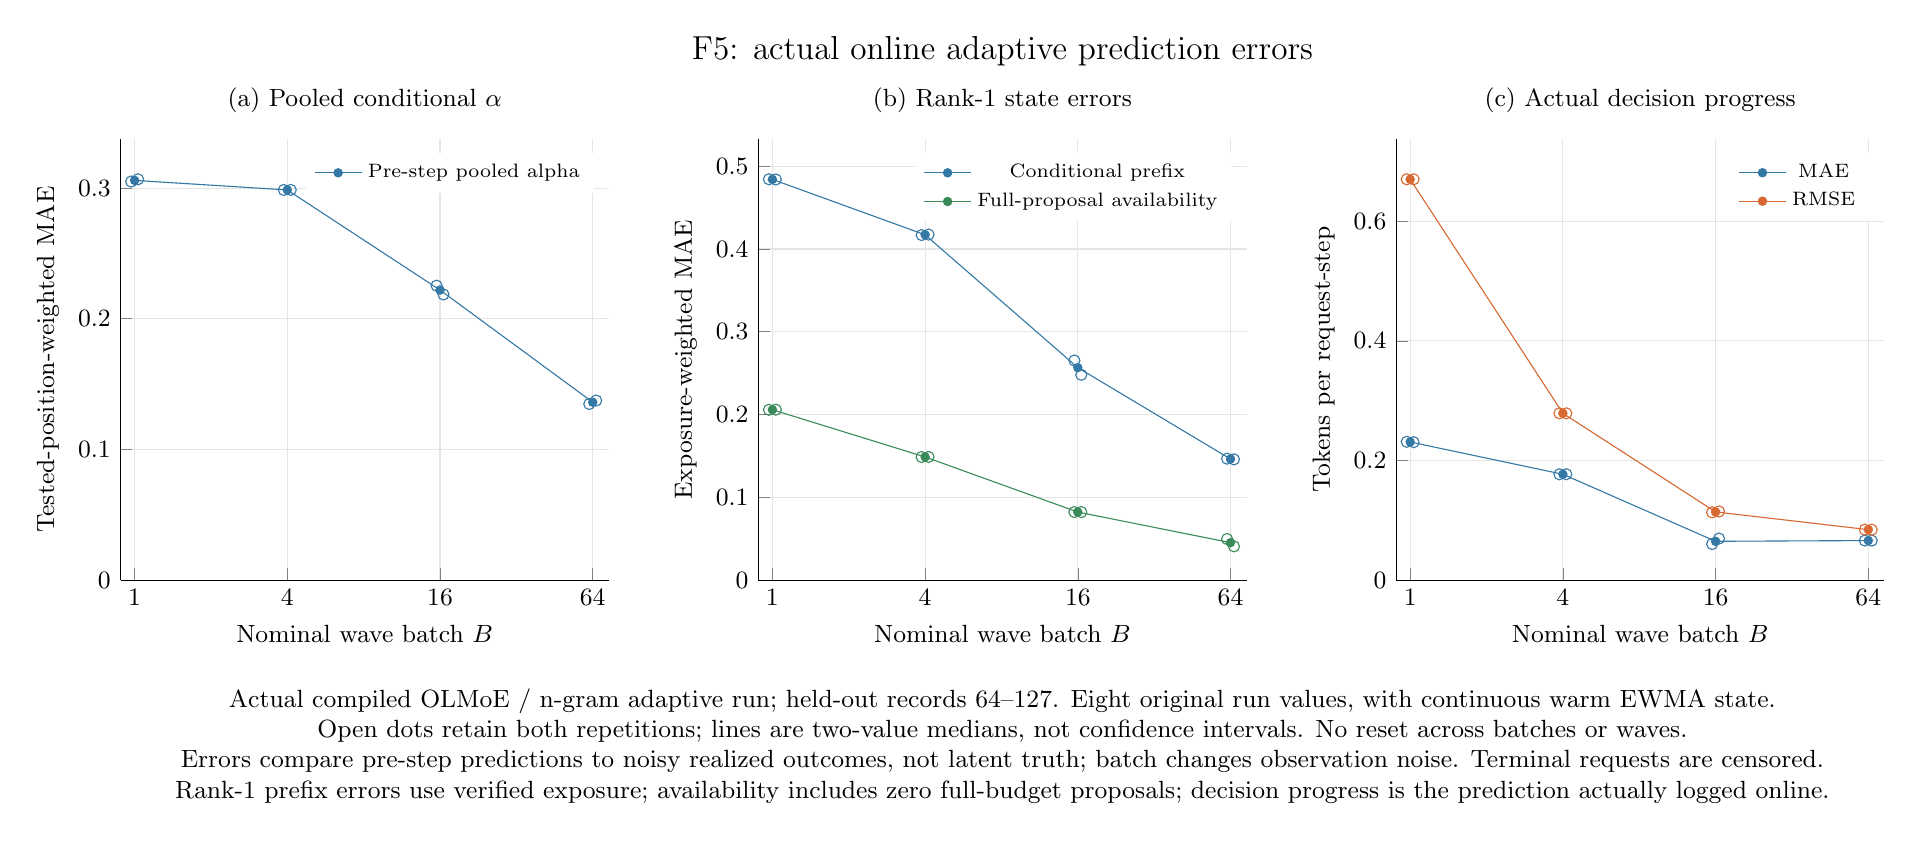
\begin{tikzpicture}
\definecolor{cal}{HTML}{3478A5}\definecolor{test}{HTML}{D76832}\definecolor{profile}{HTML}{3B8A5A}
\begin{groupplot}[group style={group size=3 by 1,horizontal sep=1.9cm},width=6.2cm,height=5.6cm,scale only axis,axis lines*=left,grid=major,grid style={gray!20},tick label style={font=\small},label style={font=\small},title style={font=\small},legend style={font=\scriptsize,draw=none},unbounded coords=jump]
\nextgroupplot[title={(a) Pooled conditional $\alpha$},ylabel={Tested-position-weighted MAE},xmode=log,log basis x=2,xtick={1,4,16,64},xticklabels={1,4,16,64},xlabel={Nominal wave batch $B$},xmin=.88,xmax=74,ymin=0,legend pos=north east]\addplot[color=cal,mark=*,mark size=1.5pt] coordinates {(1,0.305882661131) (4,0.298580478332) (16,0.22198897325) (64,0.136126952189)};\addlegendentry{Pre-step pooled alpha}
\addplot[forget plot,only marks,color=cal,mark=o,mark size=2pt,mark options={fill=white}] coordinates {(0.969289816935,0.305017287169) (1.0316831793,0.306748035093) (3.87715926774,0.298563267329) (4.12673271721,0.298597689335) (15.508637071,0.225346010109) (16.5069308688,0.218631936392) (62.0345482838,0.134798025428) (66.0277234753,0.13745587895)};
\nextgroupplot[title={(b) Rank-1 state errors},ylabel={Exposure-weighted MAE},xmode=log,log basis x=2,xtick={1,4,16,64},xticklabels={1,4,16,64},xlabel={Nominal wave batch $B$},xmin=.88,xmax=74,ymin=0,legend pos=north east]\addplot[color=cal,mark=*,mark size=1.5pt] coordinates {(1,0.484071162352) (4,0.417127635292) (16,0.256678887307) (64,0.146302974405)};\addlegendentry{Conditional prefix}
\addplot[forget plot,only marks,color=cal,mark=o,mark size=2pt,mark options={fill=white}] coordinates {(0.969289816935,0.484207408015) (1.0316831793,0.483934916689) (3.87715926774,0.416832443617) (4.12673271721,0.417422826966) (15.508637071,0.265294088713) (16.5069308688,0.2480636859) (62.0345482838,0.146746551936) (66.0277234753,0.145859396874)};
\addplot[color=profile,mark=*,mark size=1.5pt] coordinates {(1,0.205853176733) (4,0.148784914816) (16,0.0822203742496) (64,0.045254089826)};\addlegendentry{Full-proposal availability}
\addplot[forget plot,only marks,color=profile,mark=o,mark size=2pt,mark options={fill=white}] coordinates {(0.969289816935,0.205788410274) (1.0316831793,0.205917943192) (3.87715926774,0.148764567761) (4.12673271721,0.14880526187) (15.508637071,0.0822211108666) (16.5069308688,0.0822196376326) (62.0345482838,0.0497014654975) (66.0277234753,0.0408067141545)};
\nextgroupplot[title={(c) Actual decision progress},ylabel={Tokens per request-step},xmode=log,log basis x=2,xtick={1,4,16,64},xticklabels={1,4,16,64},xlabel={Nominal wave batch $B$},xmin=.88,xmax=74,ymin=0,legend pos=north east]\addplot[color=cal,mark=*,mark size=1.5pt] coordinates {(1,0.230950127299) (4,0.176974155503) (16,0.0649360757543) (64,0.0661422934518)};\addlegendentry{MAE}
\addplot[forget plot,only marks,color=cal,mark=o,mark size=2pt,mark options={fill=white}] coordinates {(0.969289816935,0.231269363289) (1.0316831793,0.230630891309) (3.87715926774,0.176895001118) (4.12673271721,0.177053309887) (15.508637071,0.0603435716947) (16.5069308688,0.069528579814) (62.0345482838,0.0661535966758) (66.0277234753,0.0661309902279)};
\addplot[color=test,mark=*,mark size=1.5pt] coordinates {(1,0.670160349343) (4,0.278895115156) (16,0.114044131067) (64,0.0844036521179)};\addlegendentry{RMSE}
\addplot[forget plot,only marks,color=test,mark=o,mark size=2pt,mark options={fill=white}] coordinates {(0.969289816935,0.670164004726) (1.0316831793,0.670156693959) (3.87715926774,0.278959206292) (4.12673271721,0.278831024021) (15.508637071,0.113303997767) (16.5069308688,0.114784264368) (62.0345482838,0.0844628143262) (66.0277234753,0.0843444899096)};
\end{groupplot}
\path (group c1r1.north west) -- node[above=0.8cm,font=\large] {F5: actual online adaptive prediction errors} (group c3r1.north east);
\path (group c1r1.south west) -- node[below=1.25cm,align=center,font=\small] {Actual compiled OLMoE / n-gram adaptive run; held-out records 64--127. Eight original run values, with continuous warm EWMA state.\\Open dots retain both repetitions; lines are two-value medians, not confidence intervals. No reset across batches or waves.\\Errors compare pre-step predictions to noisy realized outcomes, not latent truth; batch changes observation noise. Terminal requests are censored.\\Rank-1 prefix errors use verified exposure; availability includes zero full-budget proposals; decision progress is the prediction actually logged online.} (group c3r1.south east);
\end{tikzpicture}\end{document}
